\section{Chapter 9. Molecular Geometry and Bonding Theories}

\secttoc

{\footnotesize
\begin{multicols}{3}
\begin{compactenum}
    \item Predict 3D shapes using VSEPR model
    \item Polar or nonpolar based on geometry and individual dipole moments
    \item Orbital overlap and covalent bonds
    \item Hybridization atoms in molecules based on molec structures
    \item Overlap and $\sigma, \pi$ bonds.
    \item Delocalized $\pi$ bonds in molecules like Benzene
    \item Count $e^-$ in delocalized $\pi$ system
    \item Concept of bonding and antibonding MOs and draw examples of $\sigma$
        and $\pi$ MOs.
    \item MO energy-level diagram. Place $e^-$ to obtain bond orders and $e^-$
        configurations of diatomic molecules.
    \item Correlate bond order, bond strength/enthalpy, bond length,
        magnetic properties with MO descriptions of molecules.
\end{compactenum}
\end{multicols}
}

\begin{mdframed}

\subsection{Molecular Shapes}
\begin{figure}[H]
\centering
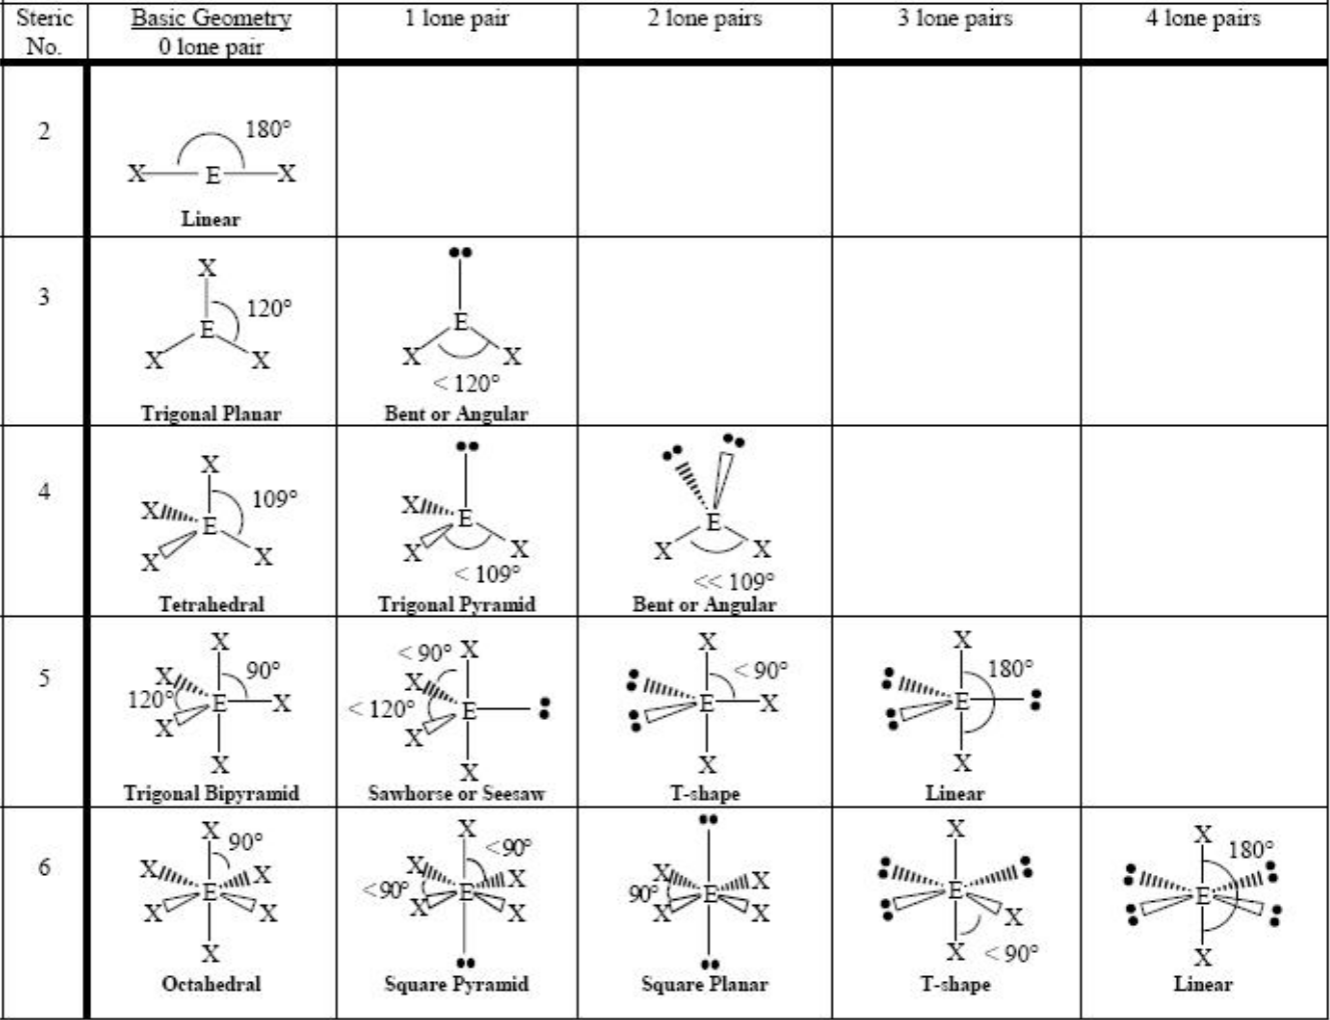
\includegraphics[width=\textwidth]{molecule_shapes.png}
\end{figure}

\subsection{VSEPR Model}
\begin{multicols}{2}
\begin{compactdesc}
\item[Shapes minimize] electron repulsion
\item[Electron Domain] a bonding pair, a multiple bond, or a non-bonding
    $e^-$. \ce{CCl2O} has 3 domains about the central atom.
\item[Nonbonding] takes up more space
\item[Multiple centers?] just find the shape for each center
\item[For 6 domains:] octahedral arrangement is the stablest
\end{compactdesc}


\end{multicols}
\end{mdframed}




\begin{mdframed}
\subsection{Covalent Bonding, Orbital Overlap}
\begin{multicols}{2}
\begin{compactdesc}
\item[Overall Polarity] of a covalent molecule. Consider the shape and each
    dipole, they may cnacel each other out, if they don't then the molecule is
    indeed polar.
\item[Combining VSEPR with Lewis] structures suggests covalent bonds form by
    the intersection of two non-bonding orbitals.
\end{compactdesc}
\begin{figure}[H]
\centering
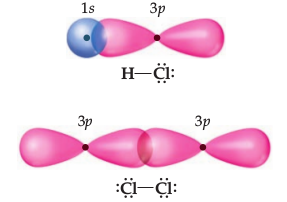
\includegraphics[width=0.3\textwidth]{orbital_overlap.png}
\end{figure}

\end{multicols}



\end{mdframed}




\begin{mdframed}
\subsection{Hybrid Orbitals}
\begin{multicols}{2}
\begin{compactdesc}
\item[Hybrid orbitals] combined atomic orbitals, have different shapes
\item[Hybridization] mixing orbitals, although number of orbitals must remain
    constant.
\item[Hypervalent] central atoms aren't generally hybridized.
\item[Linear $180^\circ$] arrangement of domains implies $sp$ hybridization.
\item[Triangular $120^\circ$] arrangement implies $sp^2$ hybridization, total 3.
\item[Tetrahedral $109.5^\circ$] arrangement implies $sp^3$ hybridization, total 4.
\item[Not all orbitals] need $s$ contact, can also be non-bonding, \ce{NH3},
    \ce{H2O} have $sp^3$ orbitals.
\item[To find] draw Lewis structure, find shapes, any $s$ orbitals? Must be
    hybrid.
\end{compactdesc}
\end{multicols}
\begin{figure}[H]
\centering
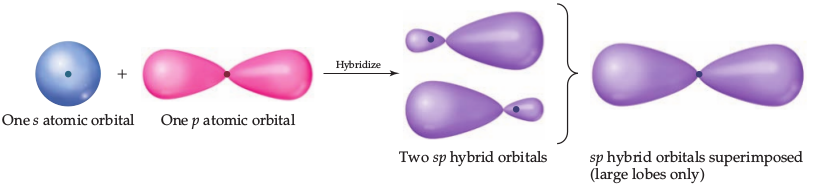
\includegraphics[width=0.9\textwidth]{sp_orbital.png}
\end{figure}

\end{mdframed}




\begin{mdframed}
\begin{multicols}{2}
\subsection{Multiple Bonds}
\begin{compactdesc}
\item[Single bonds] are called $\sigma$. Always local.
\item[Triple and double bonds] have one $\sigma$ and two or one $\pi$ bonds.
    Weaker -- roundabout for $e^-$ -- but reduces rotation.
\item[p$_\pi$ orbital] is the un-hybridized $2p$ orbital in an $sp^2$ that can
    be involved in forming a $\pi$ orbital.
\item[Benzene] rigid thanks to the \textbf{delocalized} (floating) $e^-$ in
    double bonds.
\end{compactdesc}
\begin{figure}[H]
\centering
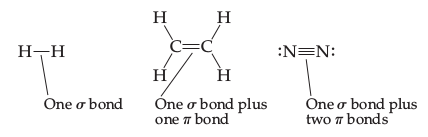
\includegraphics[width=0.4\textwidth]{sigma_pi_bonds2.png}
\end{figure}
\begin{figure}[H]
\centering
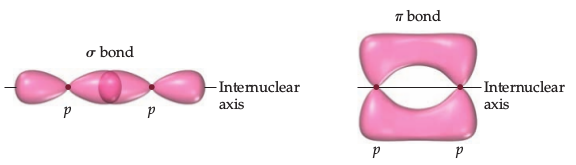
\includegraphics[width=0.45\textwidth]{sigma_pi_bonds.png}
\end{figure}
\begin{figure}[H]
\centering
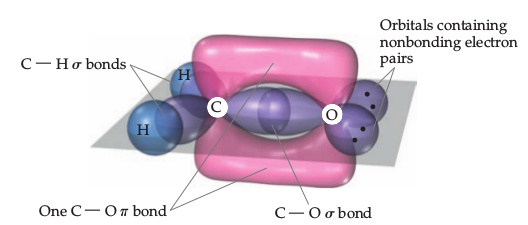
\includegraphics[width=0.45\textwidth]{h2co_orbitals.png}
\end{figure}

\end{multicols}
\end{mdframed}




\begin{mdframed}
\begin{multicols}{2}
\subsection{Molecular Orbitals}
\begin{compactdesc}
\item[Molecular orbital] wave functions describing $e^-$. Orbitals combine to
    cover the whole molecule. MO can have 0, 1 or 2 $e^-$
\item[Number of MO] number of atomic orbitals combining to make MOs.
\item[Bonding MO] waves add constructively to form mighty bond
\item[Anti-Bonding MO] waves add destructively, $e^-$ repelled.
\item[Bond order] $\frac{1}{2}$ (bonding $e^-$ - anti-bonding $e^-$).
\item[Trend:] as bond order increases, bond enthalpy increases and bond
    distance decreases
\item[Electrons arranged] according to Hund's Rule and Pauli's E. Principle.
\item[Core electrons] do not contribute to molecular bonding much
\end{compactdesc}



\subsection{Period 2 Diatomic Molecules}
\begin{compactdesc}
\item[Homonuclear diatomic] molecules (two identical)
    \begin{compactenum}
    \item number of MO = number of AO combined
    \item AO most effectively combined with other AO of similar energy
    \item Effectiveness of combo relates to overlap.
    \item MO can have two $e^-$ with opposite spin (Pauli)
    \item Hund's rule obeyed for same energy MOs
    \end{compactenum}
\item[Heteronuclear diatomic] similar to homo-nuclear, but an MO has a greater
    contribution from AO to which it is closer in energy. \ce{NO}:
    $\sigma_{2s}$ is closer to the O $2s$ than to the N $2s$, thus
    the sigma has greater contribution from O than N.
\item[Paramagnetism] unpaired $e^-$ cause magnetic attraction
\item[Diamagnetism] no unpaired $e^-$ weak magnetic repulsion
\end{compactdesc}
\end{multicols}
\end{mdframed}

\begin{mdframed}
\begin{multicols}{2}
\begin{figure}[H]
\centering
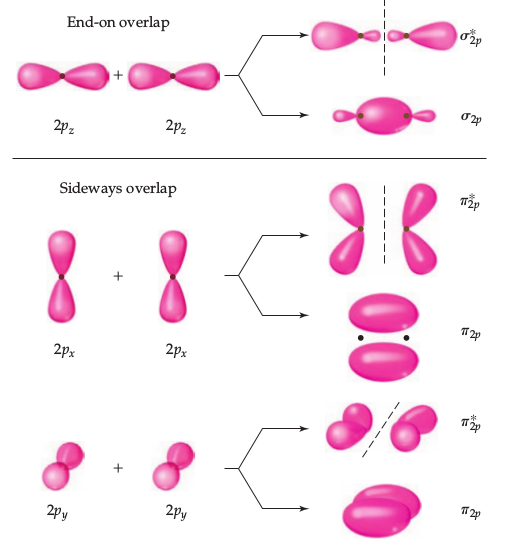
\includegraphics[width=0.45\textwidth]{2p_orbital_overlap.png}
\end{figure}


\begin{figure}[H]
\centering
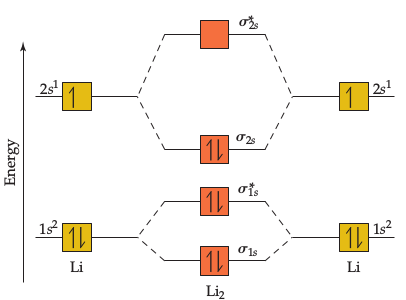
\includegraphics[width=0.40\textwidth]{li2_energy_level_diagrams.png}
\end{figure}
\begin{figure}[H]
\centering
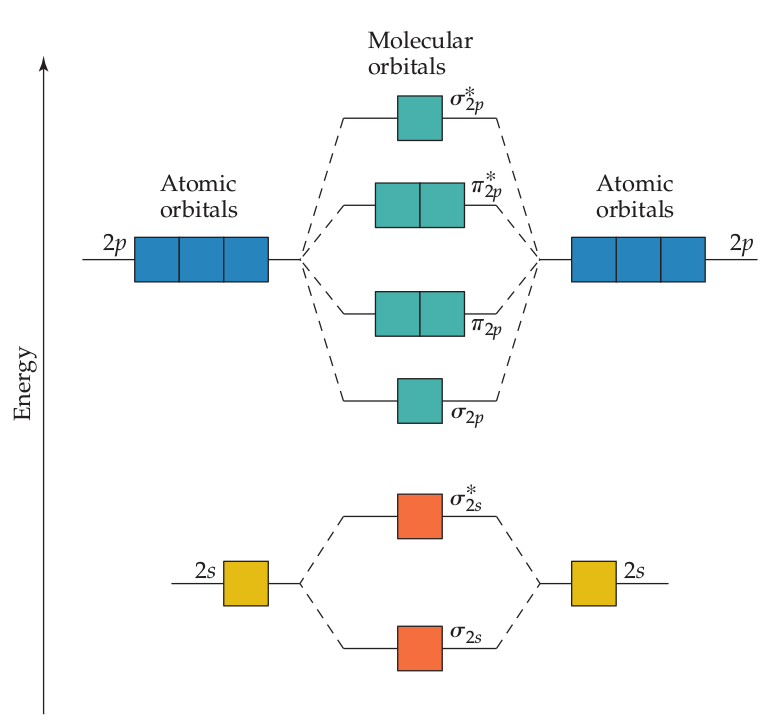
\includegraphics[width=0.45\textwidth]{period2_energy_level_diagrams.png}
\end{figure}
\begin{figure}[H]
\centering
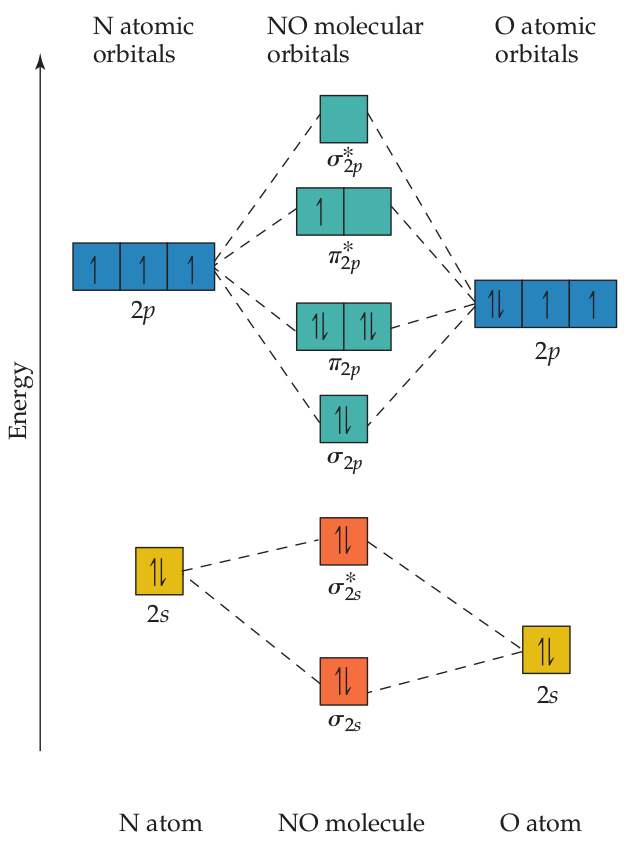
\includegraphics[width=0.45\textwidth]{no_energy_level_diagrams.png}
\end{figure}
\end{multicols}
\begin{figure}[H]
\centering
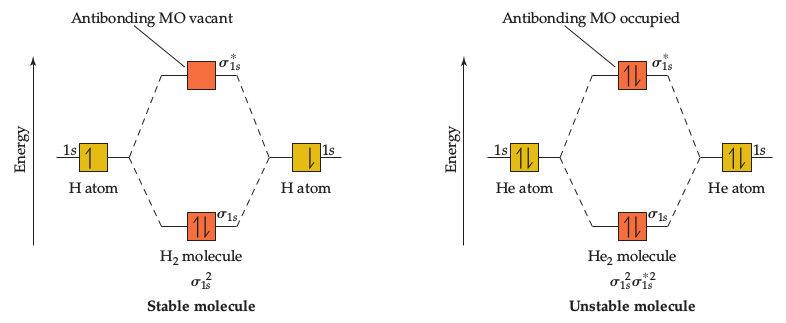
\includegraphics[width=0.8\textwidth]{h2_he2_energy_level_diagrams.png}
\end{figure}
\end{mdframed}






% Among the dead were 16 teenagers and two teachers from a German high school who had just completed a week-long exchange program in Spain. Two German opera singers also died in the crash, as did a pair of newlyweds who'd just married on Saturday. Three Americans—Yvonne Selke, 58, and her daughter, Emily Selke, 22 (pictured above); the third victim was identified by the State Department as Robert Oliver—were on board, as were citizens from Argentina, Morocco, Spain, Germany, Australia, Britain, Iran, Colombia, Kazakhstan, the Netherlands, Israel, and Japan.
